% chktex-file 46
\subsection{Water governance regimes}\label{Res.1}

\begin{figure*}[ht!]
	\centering
	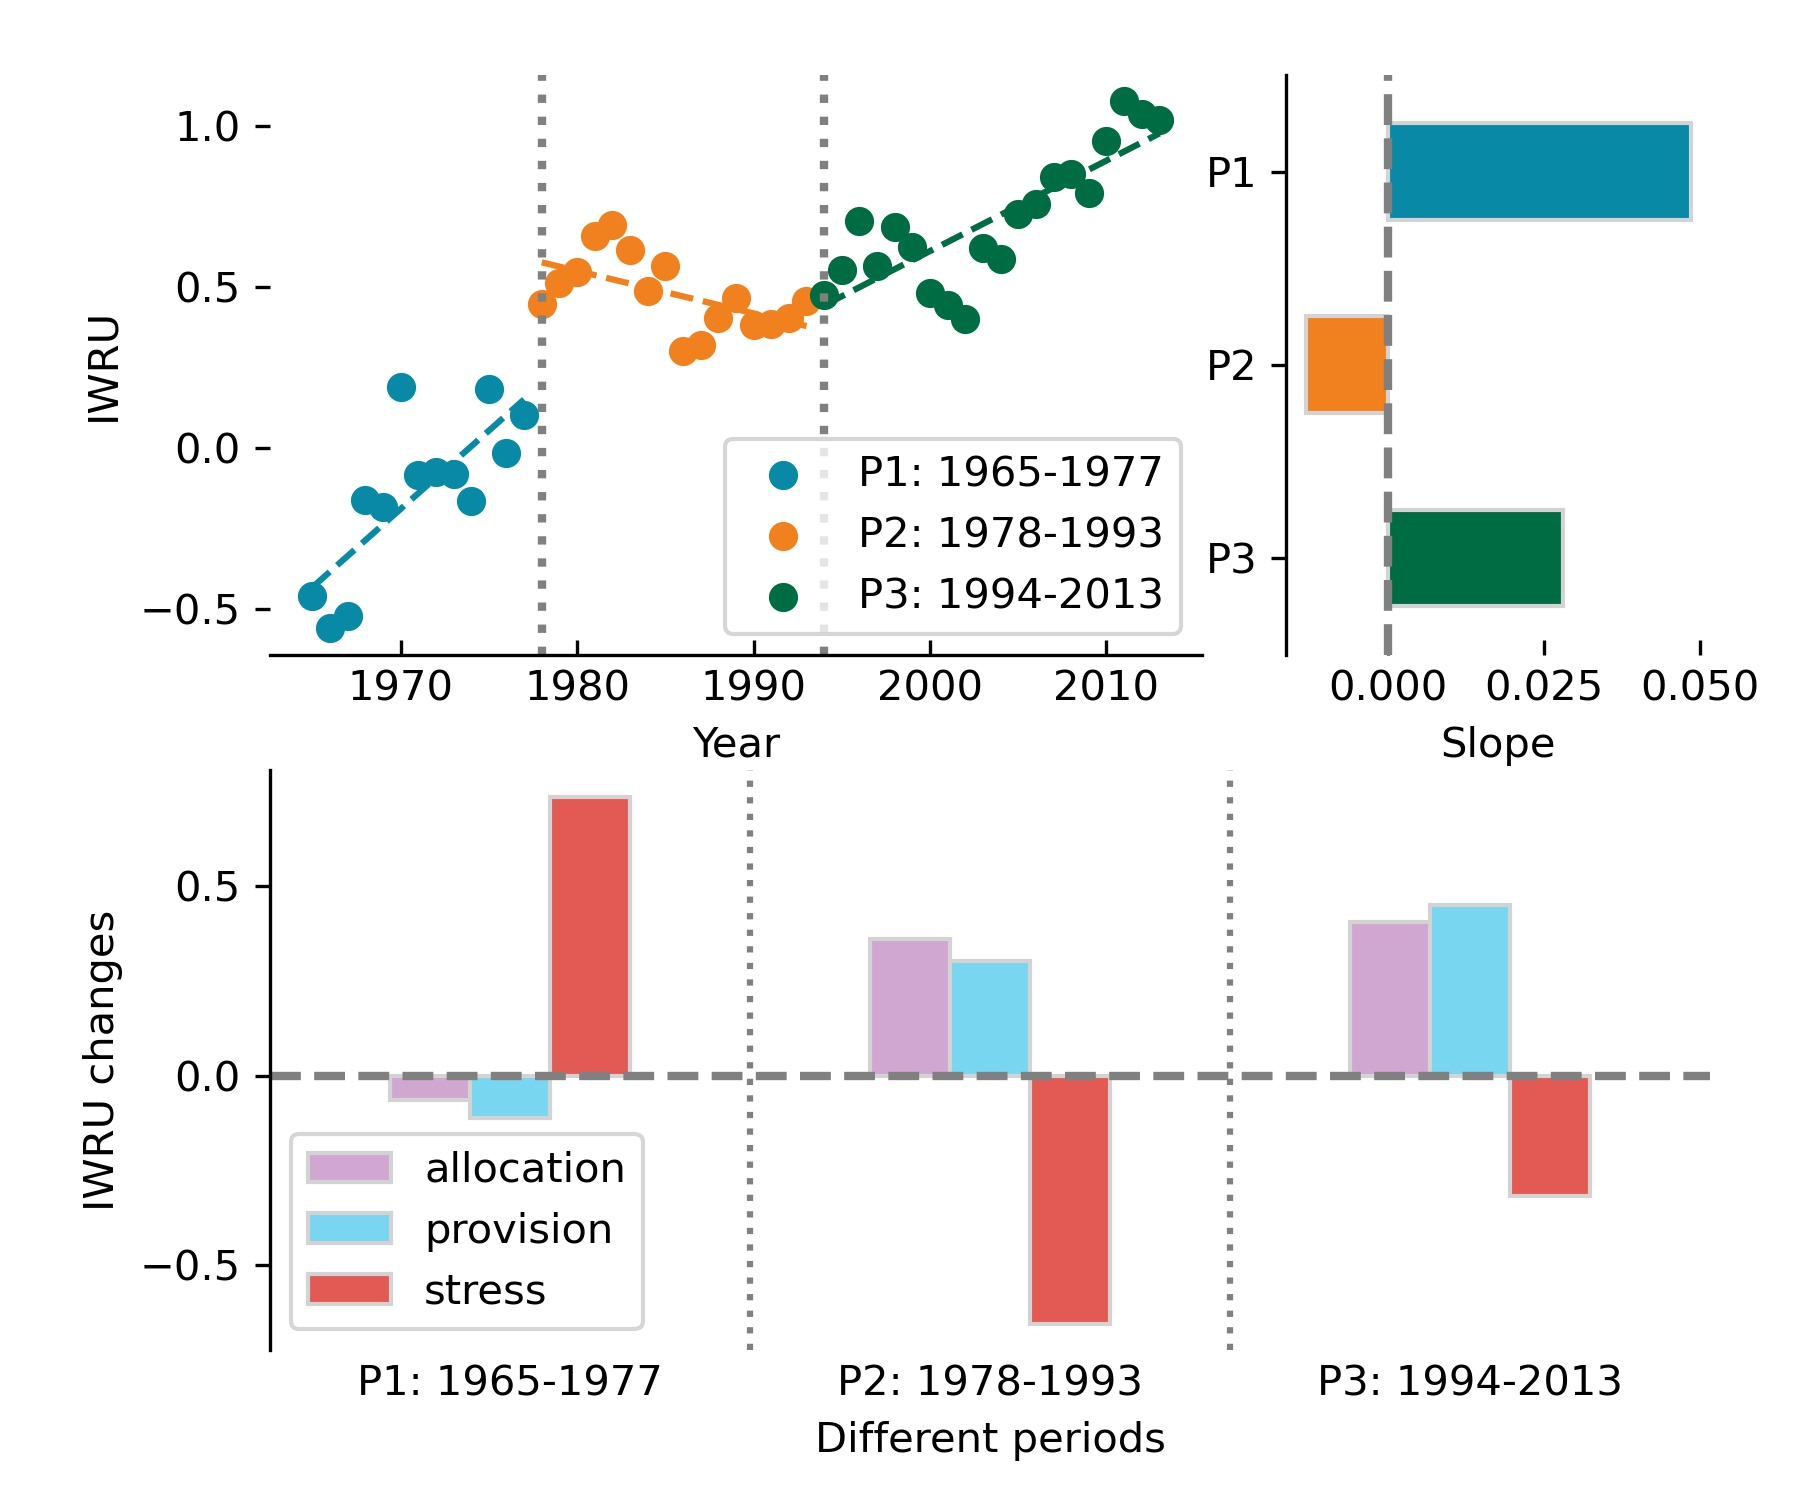
\includegraphics[width=0.9\linewidth]{main/index.jpg}
	\caption{Changes in the IWGI index and corresponding water governance regimes: P1: $1965 \sim 1978$, P2: $1979 \sim 2001$, and P3: $2002 \sim 2013$.
	\textbf{A,} detecting change points of IWGI and contributions from each indicator. Two significant change points ($p<0.001$) occurred in 1978 and 2001.
	\textbf{B,} correlation of trends between the IWGI and the indicators.
	\textbf{C,} across three indicators, changing components of the IWGI, whose directions shifts between different regimes.
	}\label{fig:IWGI}
\end{figure*}

% 这一节主要展示IWGI的变化趋势和WUR的划分
Two significant change points divide the changes in the IWGI into three periods, with different contributions from three aspects (Figure~\ref{fig:IWGI}A).
% 第一阶段
In the first period (P1, $1965 \sim 1978$), the IWGI decreased rapidly.
While the indicator of purpose and allocation contributed more to the IWGI ($49.45\%$ and $34.95\%$ on average, respectively), the remarkable downward trend correlates significantly ($p<0.01$) to the decreasing allocation and stress indicators (Figure~\ref{fig:IWGI}B).
% 第二阶段
In the second period (P2, $1979 \sim 2001$), the increasing stress indicator significantly ($p<0.01$) contributed to the upward IWGI, while the allocation and purpose indicators played negative roles in changing the IWGI.\
% 第三阶段
During the third period (P3, $1995 \sim 2013$), while the stress indicator kept its most prominent share in contributions ($57.11\%$ on average), the increased allocation indicator and decreased purpose indicator changed the regime.
% Overall
Taken together, the overall features of the three aspects in different periods are relative to a directional change in the combination of three aspects (Figure~\ref{fig:IWGI}C).

\subsection{Causes of the regime shifts}\label{Res.2}

\begin{figure*}[th!]
	\centering
	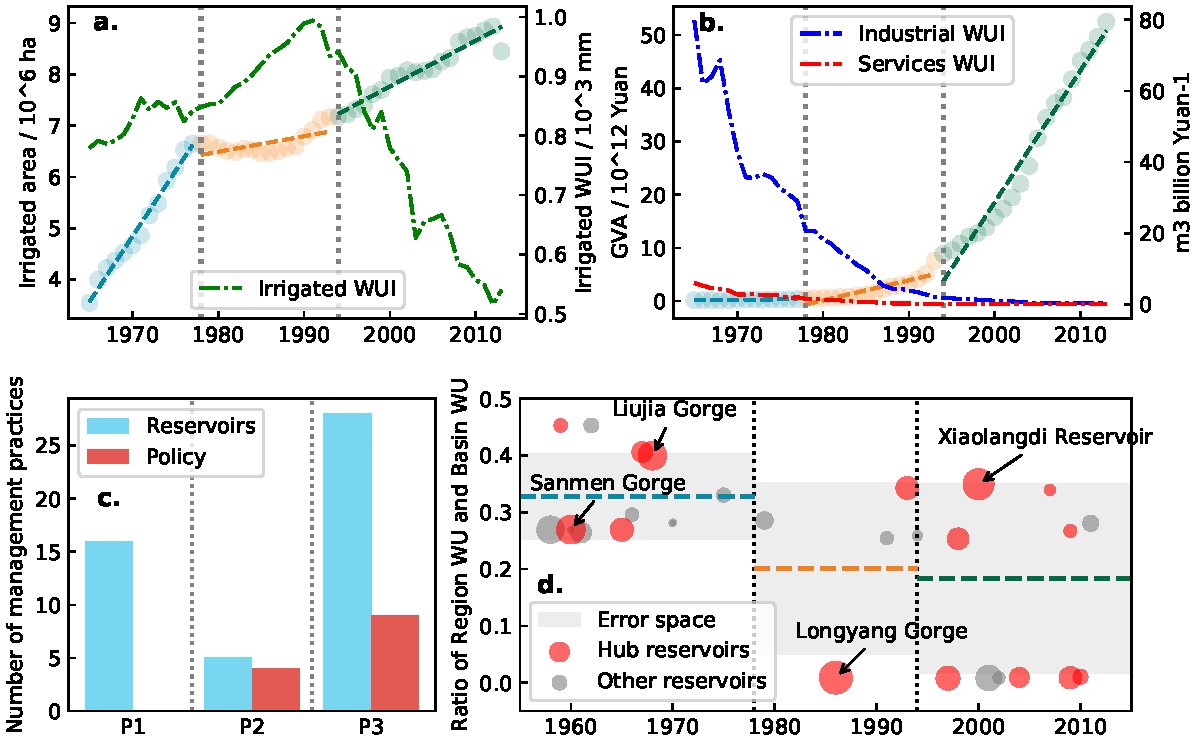
\includegraphics[width=0.9\linewidth]{main/causes.pdf}
	\caption{
		Causes of water governance regime shifts in the YRB.\
		\textbf{A.} Changes in the total irrigated area (orange line) and water use intensity ($WU/A$, water use divided by the irrigated area, the green dot line).
		\textbf{B.} Changes in gross values added (GVA) of industry and services (blue line) and their water use intensities ($WU/GVA$ WU divided by the GVA, the red dot line).
		\textbf{C.} Completed time of each new reservoir and their located region's water use (LWU) percentages as a proportion of the total basinal water use (BWU) at that time. Dashed lines denote average of these percentages in different regimes. Red circles (Major Reservoirs) denote the reservoirs mainly for managing and regulating the whole basin.
		The size of each circle indicates the magnitude of its water storage capacity.
		\textbf{D.} Social atmosphere$^*$ (red triangles) and national-level governance policies (the circles, different colours denote signed by different state agencies). The light grey bars count official documents related to the YRB on a basinal scale (the Yellow River Events).
		\footnotesize{$^*$ Here, ``social atmosphere'' refers to the sociocultural context in which people live or in which something happens, including the culture that the individual was educated or lives.}
	}\label{fig:Causes}
\end{figure*}

% 进一步挖掘IWGI变化的根本原因,
The underlying causes of changes in the IWGI are different in the two regime shifts.
% 灌溉区扩张和工业和服务业的经济增长是P1和P2目的变化的关键。
Changing water demands and supply were critical to the shift between P1 and P2.
% P1年,黄河流域灌溉农业面积以图A的速度快速扩张,灌溉用水占主导(1965年占总用水的$81.56\%$, 1978年占总用水的$83.17\%$,图S3)。
As the dominant water demand during the P1, the area of irrigated agriculture in the YRB expanded rapidly at a rate of $0.25*10^6~ha/yr$ (Figure\ref{fig:Causes}~A), simultaneously supported by increasing supply through the construction of reservoirs.
% 然而,进入P2后,灌溉区扩张停滞,工业和服务业逐渐增长,用水需求增加(图re\ref{fig: Causes} B),导致灌溉用水量比例下降$8\%$ S3。
Ensuing the P2, however, the expansion of irrigated areas slowed down, and industry and services gradually took off (Figure\ref{fig:Causes}~A and B).
% 水分利用效率由P2变化到P3。
Then, the efficiency of water use changed obviously from P2 to P3.
Not only did irrigated areas continue to expand slowly during the P3 (Figure\ref{fig:Causes}~A), but industry and urban services also assumed a more vital economic role (represented by Gross Added Values, GVA) (Figure~\ref{fig:Causes}~B).
Because of increased efficiency, however, they both experienced significant declines in water use for a unit irrigated area or unit production (Figure~\ref{fig:Causes}~A and Figure~\ref{fig:Causes}~B).
As a result, the differences between sectors and regions in water use reduced while the total water stress steadily remained high during the P3 (Figure~\ref{fig:IWGI}A).

% 最后,环境背景、社会转型和水治理政策在这三个时期都发挥了作用。
Environmental and social contexts, governance policies played roles in all three periods.
We calculated the ratios of regional and basinal water use for each reservoir (R/B ratio) (Figure~\ref{fig:Causes}C), with a higher ratio representing a potential role in water supply rather than basinal regulations.
Under the banner of ``conquering nature'' most of the reservoirs were built in regions with high water demands during the P1 (R/B ratios were significantly higher ($p<0.01$, see Figure~\ref{fig:Causes}C)).
Ensuing the P2, the number of new reservoirs decreased but boosted their role in water regulating and management (more red circles in Figure~\ref{fig:Causes}~C, and larger water conveyance variability in Supporting Informations Figure~S8).
Basin policies significantly increased, rigorously controlled the allocation of water (Figure~\ref{fig:Causes}D, $p<0.01$).
During the P3, authorities proposed more national-level water governance policies under the guidance of the national strategy ``environmental regulation'' (Figure~\ref{fig:Causes}D).
The regime shift from P1 to P2 is in line with the increasing water supply and demands; while driven by regulatory policies and efficiency enhancement under stable water stress from P2 to P3.
